\section{The Magic Gem}
\label{sec:gem}

Let $S=(s_{ij})$ be an arrangement of order $n\ge2$, with cells indexed by $i,j\in\{0,\dots,n-1\}$ ($i$ the row from the top, $j$ the column from the left), and write $N=n^2$ and $\bar s=(N+1)/2$ for the mean entry.

\begin{definition}[Gem coordinates and Magic Gem]
\label{def:gem_coords}
To the cell $(i,j)$ assign the point $\mathbf p_{ij}=(x_{ij},y_{ij},z_{ij})\in\R^3$ with
\begin{equation}
x_{ij}=j-\frac{n-1}{2},\qquad y_{ij}=\frac{n-1}{2}-i,\qquad z_{ij}=s_{ij}-\bar s.
\label{eq:gem_coords}
\end{equation}
The \emph{Magic Gem} of $S$ is the convex hull $\mathcal G(S)=\operatorname{conv}\{\mathbf p_{ij}\}$, and $z=(z_{ij})$ is the \emph{height function} of $S$.
\end{definition}

The $x$-axis runs along the columns and the $y$-axis along the rows (top row at positive $y$).
Let $x_j=j-\frac{n-1}2$ and $y_i=\frac{n-1}2-i$ denote the $n$ values taken by $x$ and $y$.
A \emph{line} is one of the $n$ rows, the $n$ columns, the main diagonal $\{i=j\}$ or the anti-diagonal $\{i+j=n-1\}$.
For a line $L$ let $\delta_L(S)=\sum_{c\in L}s_c-\mu_n$ be its \emph{deviation}, so $S$ is magic iff $\delta_L(S)=0$ for all $2n+2$ lines.
Moment and centroid statements below refer to the $N$ points $\mathbf p_{ij}$ with unit weights, not to the solid $\mathcal G(S)$.

\paragraph{Terminology.}
Each point $\mathbf p_{ij}$ is either a \emph{vertex} of $\mathcal G(S)$, an \emph{interior point} (in the interior of $\mathcal G(S)$), or a \emph{boundary non-vertex point} (on the boundary but not a vertex).
We write $\operatorname{vert}\mathcal G(S)$ for the vertex set, $V$, $V^\circ$, $V^\partial$ for the three numbers ($V+V^\circ+V^\partial=N$), $V/N$ for the \emph{vertex fraction}, and $(V,E,F)$ for the $f$-vector.
Facets are denoted $\Gamma$.
For any set $X\subseteq\R^3$, $\operatorname{Iso}(X)$ is the group of isometries of $\R^3$ that map $X$ onto itself.
The dihedral group $D_4=\langle r,h\rangle$ of the square acts on arrangements by $(gS)_{gc}=s_c$; here $r$ is the quarter-turn, $r^2$ the half-turn, $h$ and $v$ the left--right and top--bottom reflections and $t$ the transpose.
For $g\in D_4$ let $\hat g(x,y,z)=(g(x,y),z)$, where $g$ acts on the plane as the corresponding orthogonal map.
The order-four squares are numbered $\#0,\dots,\#879$ in the lexicographic order of their Fr\'enicle standard forms (the image under $D_4$ with the smallest corner entry at top left and $s_{01}<s_{10}$) \cite{frenicle1693}; the list is \texttt{anc/squares880.txt}.

\begin{lemma}[Means, variances, line sums]
\label{lem:lines}
For every arrangement $S$ of order $n$:
\begin{enumerate}
\item $\sum_{i,j}x_{ij}=\sum_{i,j}y_{ij}=\sum_{i,j}z_{ij}=0$ and $\sum_{i,j}x_{ij}y_{ij}=0$;
\item $\frac1N\sum x_{ij}^2=\frac1N\sum y_{ij}^2=a_n:=\frac{n^{2}-1}{12}$ and $\frac1N\sum z_{ij}^2=b_n:=\frac{N^{2}-1}{12}$;
\item for every line $L$, $\delta_L(S)=\sum_{c\in L}z_c$, and
$\sum_{c\in L}\mathbf p_c=\bigl(n\,\bar x_L,\ n\,\bar y_L,\ \delta_L(S)\bigr)$,
where $(\bar x_L,\bar y_L)$ is the centre of the line: $(0,y_i)$ for the row $i$, $(x_j,0)$ for the column $j$, and $(0,0)$ for both diagonals.
\end{enumerate}
In particular $S$ is magic if and only if the vector sum of the $\mathbf p_c$ along every line is horizontal.
\end{lemma}

\begin{proof}
(1) $\sum_{i,j}x_{ij}=n\sum_j x_j=0$, likewise for $y$; $\sum z=\sum_{k=1}^{N}k-N\bar s=0$; and $\sum xy=(\sum_jx_j)(\sum_iy_i)=0$.
(2) $\frac1n\sum_jx_j^2$ is the variance of $n$ equally spaced points with unit spacing, $(n^2-1)/12$; the same holds for $y$, and for $z$ with $N$ points.
(3) Since $\mu_n=n\bar s$, $\sum_{c\in L}z_c=\delta_L$. The cells of row $i$ have $y=y_i$ and $x$ running over all $x_j$; for a column the roles are exchanged; each diagonal is invariant under $(x,y)\mapsto(-x,-y)$.
\end{proof}

\begin{figure}[htbp]
\centering
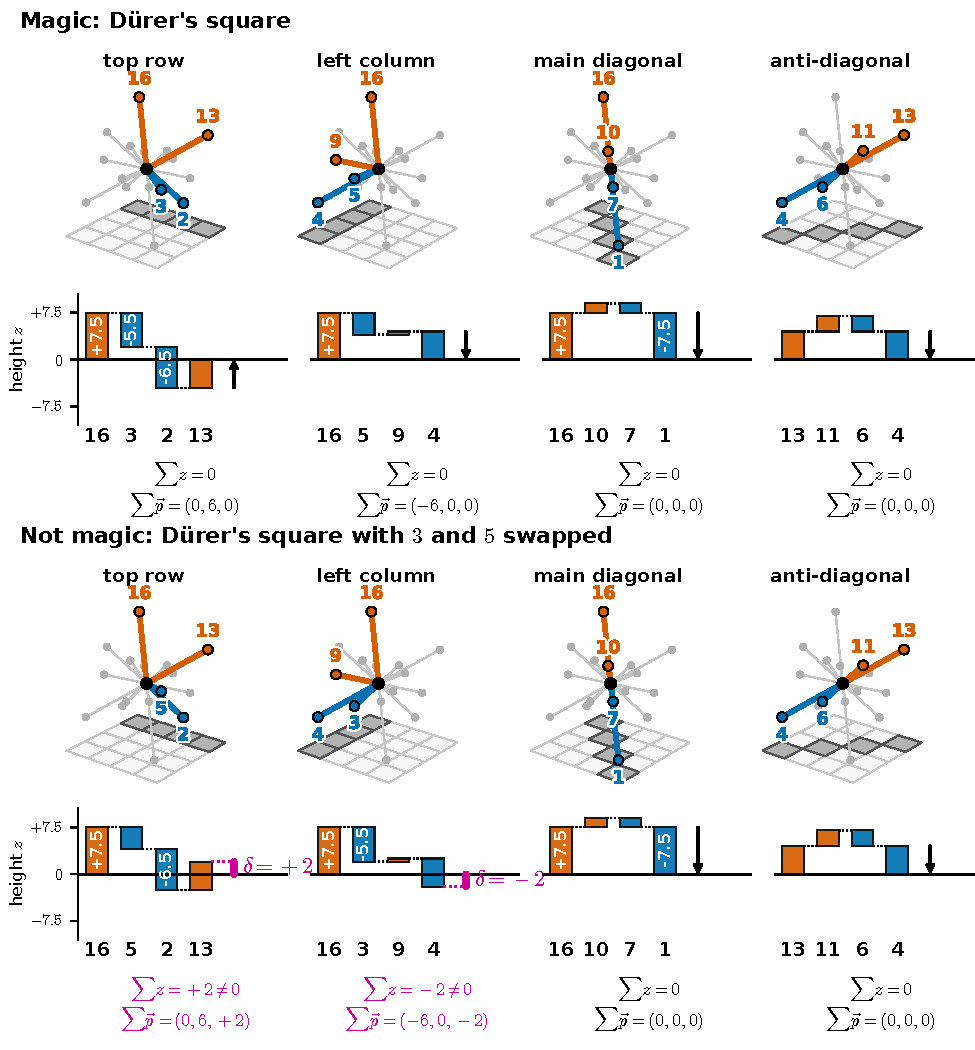
\includegraphics[width=0.92\textwidth]{figures/fig_lines.pdf}
\caption{Heights cancel along every line. \emph{Top:} for D\"urer's square, the vectors of the top row, left column and both diagonals (coloured; the cells of the line shaded on the floor), and below each the heights $z=s-8.5$ of the line stacked head to tail; the running total returns to $0$, so $\sum_{c\in L}\mathbf p_c$ is horizontal (\Cref{lem:lines}(3)). \emph{Bottom:} after swapping the entries $3$ and $5$ the top row and the left column no longer close (deviations $\delta_L=\pm2$, magenta); the diagonals do not contain the swapped cells.}
\label{fig:lines}
\end{figure}

For $g\in D_4$ the points of $gS$ are $\hat g\,\mathbf p_c$, so
\begin{equation}
\mathcal G(gS)=\hat g\,\mathcal G(S),
\label{eq:d4}
\end{equation}
and since $D_4$ maps magic squares to magic squares, every $D_4$-class of magic squares has a single gem up to congruence.

\begin{proposition}[Dimension]
\label{prop:fulldim}
Let $S$ be an arrangement of order $n\ge2$.
The points $\mathbf p_{ij}$ are coplanar if and only if $S$ is one of the eight $D_4$-images of the row-by-row arrangement $s_{ij}=ni+j+1$.
Otherwise $\mathcal G(S)$ is a $3$-polytope with the origin in its interior.
In particular this holds for every semi-magic square.
\end{proposition}

\begin{proof}
The grid positions are not collinear, so a plane containing all points is not vertical and the points are coplanar if and only if $z=\alpha x+\beta y+\gamma$ on the grid.
Then $u=\alpha$ and $w=-\beta$ are the differences of the entries of horizontally and vertically adjacent cells, so they are integers, and $s_{ij}=s_{00}+uj+wi$.
Since the entries are distinct, $u,w\ne0$; applying $h$, $v$ and $t$ we may assume $1\le u\le w$, so that $s_{00}=1$ is the smallest entry.
The entry $2$ is $1+uj+wi$ with $(i,j)\ne(0,0)$, hence $u=1$, and row $0$ holds $1,\dots,n$.
The entry $n+1$ lies in a row $i\ge1$, so $w\le n$; if $w<n$ then the cells $(0,w)$ and $(1,0)$ both hold $1+w$.
Hence $w=n$ and $s_{ij}=ni+j+1$; conversely, every $D_4$-image of this arrangement has affine heights.
If the points span $\R^3$ affinely, their centroid, which is $\mathbf 0$ by \Cref{lem:lines}(1), is a convex combination with positive weights of all of them and hence an interior point of the hull.
Finally, if $S$ is semi-magic and $z=\alpha x+\beta y+\gamma$, then $\gamma=0$ by \Cref{lem:lines}(1), the row $i$ has height sum $n\beta y_i=0$ for all $i$ and the column $j$ has $n\alpha x_j=0$, so $\alpha=\beta=0$, which is impossible.
\end{proof}

The row-by-row arrangement of order $3$ shows that the hypothesis is needed: its gem is a parallelogram.

\begin{example}[Lo Shu]
\label{ex:loshu}
For the Lo Shu square $S=\begin{pmatrix}2&7&6\\9&5&1\\4&3&8\end{pmatrix}$, $\bar s=5$ and the nine points are
\[
\begin{array}{lll}
\mathbf p_{00}=(-1,1,-3), & \mathbf p_{01}=(0,1,2), & \mathbf p_{02}=(1,1,1),\\
\mathbf p_{10}=(-1,0,4), & \mathbf p_{11}=(0,0,0), & \mathbf p_{12}=(1,0,-4),\\
\mathbf p_{20}=(-1,-1,-1), & \mathbf p_{21}=(0,-1,-2), & \mathbf p_{22}=(1,-1,3).
\end{array}
\]
The origin is the only non-vertex point and is interior; the gem has $f$-vector $(8,16,10)$ and volume $18$ (\Cref{fig:construction}).
\end{example}

\begin{figure}[htbp]
    \centering
    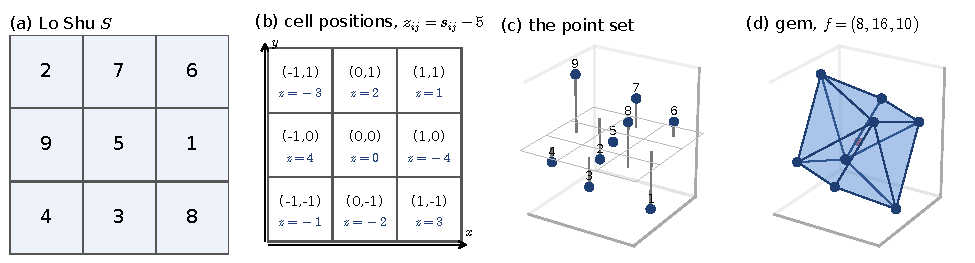
\includegraphics[width=\textwidth]{figures/fig_construction.pdf}
    \caption{The gem of the Lo Shu square: (a)~the square; (b)~the centred cells $(x_{ij},y_{ij})$ with the heights $z_{ij}=s_{ij}-5$; (c)~the nine points, labelled by the entries; (d)~their convex hull, with $f$-vector $(8,16,10)$ and the interior point $\mathbf 0$.}
    \label{fig:construction}
\end{figure}

\subsection{Gems and regular subdivisions}
\label{sec:subdivisions}

Let $A$ be the $n\times n$ grid of cell positions.
For a height function $\omega\colon A\to\R$, the \emph{regular subdivision} $\mathcal S(\omega)$ of $A$ is obtained by projecting to the plane the lower faces of $\operatorname{conv}\{(c,\omega(c))\}$, i.e.\ the faces whose outer normals have negative last coordinate; its cells are the sets of grid points whose lifts lie on a common lower face \cite[Ch.~2]{deloera2010triangulations}, \cite[Ch.~7]{gelfand1994discriminants}.
$\mathcal S(\omega)$ does not change if $\omega$ is multiplied by a positive scalar or an affine function of $(x,y)$ is added to it; the height functions inducing a given subdivision form a relatively open polyhedral cone, its \emph{secondary cone}.
By definition, $\mathcal G(S)$ is the lift of $A$ by the height function $z$ of $S$, and its upper faces are the reflections in $z=0$ of the lower faces of the lift by $-z$.

\begin{proposition}[Gems as pairs of regular subdivisions]
\label{prop:subdivisions}
Let $S$ be an arrangement of order $n\ge2$ that is not a $D_4$-image of the row-by-row arrangement.
\begin{enumerate}
\item Every facet of $\mathcal G(S)$ is a lower facet, an upper facet or a vertical facet. Projection to the plane maps the lower facets onto the maximal cells of $\mathcal S(z)$ and the upper facets onto the maximal cells of $\mathcal S(-z)$.
\item The vertical facets lie in the four planes $x=\pm\frac{n-1}2$, $y=\pm\frac{n-1}2$; the plane over a side of the grid contains a facet if and only if the entries along that side, in cell order, are not an arithmetic progression.
\item $\mathbf p_c$ is a vertex of $\mathcal G(S)$ if and only if $c$ is a vertex of a cell of $\mathcal S(z)$ or of $\mathcal S(-z)$.
\item The face lattice of $\mathcal G(S)$, with vertices labelled by cells, is determined by the pair $(\mathcal S(z),\mathcal S(-z))$, hence by the secondary cones containing $z$ and $-z$. The complement $N+1-S$ exchanges the two subdivisions.
\end{enumerate}
\end{proposition}

\begin{proof}
(1) is the definition of $\mathcal S(\pm z)$.
(2) A vertical facet lies in a plane $\ell(x,y)=\max_A\ell$ for a linear form $\ell$; the maximisers of $\ell$ on the grid are a corner or the $n$ cells of a side, and the face is $2$-dimensional only in the second case and only if the lifts of the side are not collinear, i.e.\ if the heights along the side are not an affine function of the position.
(3) The vertical line through a vertex $\mathbf v$ meets $\mathcal G(S)$ in a segment with endpoint $\mathbf v$, so $\mathbf v$ lies on a lower or an upper face, of which it is a vertex; conversely the vertices of a face are vertices of the polytope.
(4) The lower and upper faces together with their incidences are read off from the two subdivisions, and by (2) the vertical facets are the polygons over the sides on which the lower and upper boundary chains differ.
The complement has height function $-z$.
\end{proof}

In this language the corner points of the grid, which are vertices of $\operatorname{conv}A$, are vertices of every gem, lying on both the lower and the upper hull, and the other forced vertices of \Cref{lem:forced} are the lowest and the highest lifted point over each edge of $\operatorname{conv}A$, which are vertices of the restrictions of $\mathcal S(z)$ and $\mathcal S(-z)$ to that edge.
For the $880$ order-four gems, $856$ have four vertical facets, $20$ have three and $4$ have two; the height functions of the $7040$ order-four magic squares induce $417$ distinct regular subdivisions of the $4\times4$ grid up to $D_4$, and for $548$ of the $880$ classes $\mathcal S(z)$ is a triangulation (\texttt{anc/verify\_revision.py}).
The census of combinatorial types in \Cref{sec:census} thus records which pairs of secondary cones of the $4\times4$ grid contain the pairs $(z,-z)$ for height functions $z$ of magic squares, and the Siamese theorem of \Cref{sec:siamese-gems} is the computation of $\mathcal S(\pm z)$ for one infinite family, made possible by the invariance of $\mathcal S$ under adding affine functions.
